% !TeX root = ../libro.tex
% !TeX encoding = utf8

\chapter{Red Neuronal}
\section{El problema de clasificar una imagen.}

Cuando observamos una imagen, podemos localizar varios elementos a partir de los cuáles esta se encuentra compuesta con tan sólo un vistazo. Sin embargo, para un ordenador no se trata de algo tan sencillo puesto que para él se trata de un gran conjunto de números que no tienen por qué tener relación alguna entre sí.\\

\begin{figure}[htpb]
  \centering
  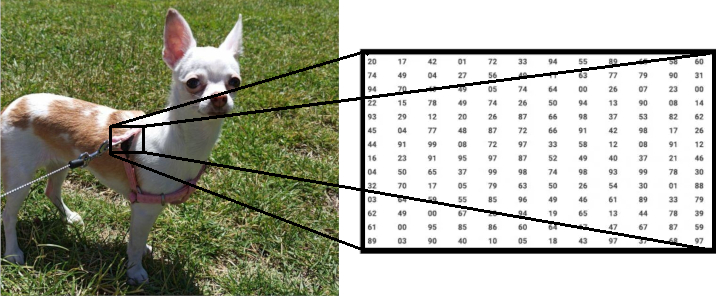
\includegraphics[width=0.8\textwidth]{blanquita}
  \caption{Cómo un ordenador ve una imagen}
  \label{fig:blanquita}
\end{figure}

Idealmente, en esta imagen desearíamos que fuera capaz de identificar que se trata de un perro, en concreto de un chiguagua, de pelaje blanco y manchas color café que se encuentra sobre un césped. Estos poquitos datos que para nosotros parecen tan triviales necesitan de horas y horas de computación para ser obtenidos a partir de una imagen cualquiera.\\

Dejamos todos estos detalles, a los cuales esperamos poder llegar en un futuro no muy lejano, y simplificamos el problema a tener un conjunto de etiquetas y buscar con cuál de todas ellas tiene mayor relación nuestra imagen.\\

Una primera idea, sería utilizar utilizar \emph{$k$-Nearest Neighbor Classifier}, en adelante $k$-NN. Este clasificador consiste en que para cada etiqueta se correspondan $k$ imágenes y consideraremos como etiqueta idónea para nuestra clasificación aquella cuya distancia, siendo Manhattan y Euclídea las más comunes, entre los píxeles con nuestra imagen sea menor. Nos encontramos con que el tiempo de entrenamiento de nuestro clasificador sería ínfimo en comparación con el tiempo de clasificación, si bien se pueden hacer diversas mejoras que cambien estos hechos. \\

De esta sencilla propuesta, surgen diversos problemas. Al darle mayor importancia al valor concreto de los píxeles, en lugar de a las formas que de las que está compuesta la figura, nos encontramos con que valores como los colores de fondo pueden influir más en la clasificación que los propios píxeles de la figura que queremos clasificar. En el ejemplo de la imagen del chiguagua, si considerásemos las etiquetas verde y perro, tendríamos que por lo general como respuesta el color verde, pese a que estamos más interesados por la mascota en sí. Otro gran problema, sería la baja escalabilidad que nos proporciona esta solución, al incrementarse enormemente el costo computacional de clasificación conforme aumenta el número de etiquetas.\\

El siguiente paso, es buscar una forma de ``memorizar'' los datos de entrenamiento de forma que no tengamos que estar comparándolos con todos ellos cuando queramos clasificar una imagen. Lo que buscamos es poder valorar de alguna forma la imagen completa y a partir de esta ``puntuación'' conocer qué etiqueta le corresponde mejor a nuestra imagen. De esta forma, veríamos drásticamente reducido el tiempo de clasificación, sacrificando para ello el tiempo de entrenamiento, y podríamos ampliar en varias unidades la cantidad de datos de entrenamiento utilizados, aumentando así la precisión de nuestro clasificador.
